%\documentclass[12pt, a4paper]{scrartcl}
%\usepackage[ngerman]{babel}
%\usepackage[utf8]{inputenc}

%\begin{document}
\section{Entwurf und Umsetzung der Netzwerk-Schnittstelle}
\subsection{Grundlegende Theorie zur Kommunikation in einem Netzwerk}
Unter dem Begriff Netzwerk im Zusammenhang mit dieser Arbeit wird, sofern es nicht ausdrücklich anders definiert ist, die Ansammlung mehrerer, untereinander verbundener Computer verstanden.
Diese haben die Möglichkeit mit standardisierten Internet-Netzwerkprotokollen miteinander zu kommunizieren.\\ 

\begin{wrapfigure}{r}{.55\textwidth}
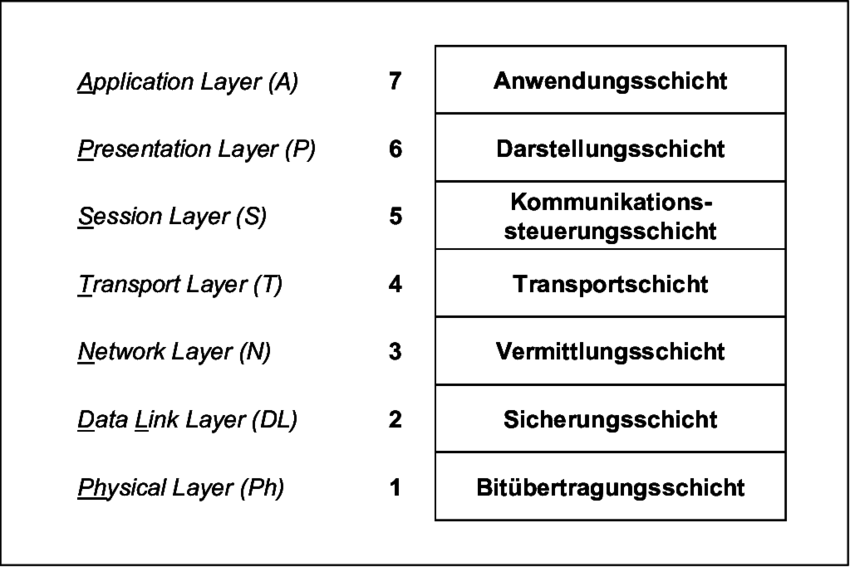
\includegraphics[scale=1]{isoosi}
\caption{Schematischer Aufbau des ISO/OSI-Modells\protect\footnotemark}
\label{ISOOSI}
\end{wrapfigure}
\footnotetext{https://www.researchgate.net/profile/Sebastian\_Lempert/publication/202268228/figure/fig1/\\AS:393996175200256@1470947416022/Abbildung-1-Die-7-Schichten-des-ISO-OSI-Referenzmodells-Der-geschichtete-Aufbau-eines.png}

Diese Kommunikation wird beschrieben durch das ISO/OSI Modell der Netzwerkkommunikation, auf dem auch die Arbeitsweise unseres Programmes aufbaut.
Innerhalb dieses Modells kann man den Prozess einer Netzwerkübertragung sowie die dabei verwendeten Informationen bzw. Protokolle in Schichten nach ihrem Abstraktionsgrad einteilen, von Nullen und Einsen in einem Kabel bis hin zu z.B. verschiedensten Verschlüsselungsprotokollen; was in unteren Schichten abgesichert ist, muss in denen darüber nicht implementiert werden, was wiederum zu einfachen und verlässlichen einzelnen Algorithmen in einer Schicht führt, obwohl das gesamte System überaus komplex ist. 
Das Modell ist in Abbildung \ref{ISOOSI} dargestellt.

\subsection{Notwendigkeit, Anforderungen und Spezifikation eines eigenen Netzwerkprotokolls}
Um das Programm zu dritt zu entwickeln, muss eine gewisse Modularität gewährleistet werden, außerdem müssen die Sinnabschnitte klar nach ihrer Funktion gegliedert sein und leicht benutzbare sowie wiederverwendbare Schnittstellen besitzen, damit nicht das gesamte Programm angepasst werden muss, wenn ein Teil geändert wird und jeder sich auf seinen Teil konzentrieren kann, ohne die anderen vollständig zu kennen.
Diese Anforderung wird durch die Trennung der Programmiersprachen Lua und C++ einfach geregelt, aber in reinem C++ Kontext muss es dennoch eine Unterteilung zwischen Netzwerkschnittstelle und Benutzeroberfläche geben, weshalb die gesamte Netzwerkkommunikation über eine statische Bibliothek in die ausführbare Datei eingebunden ist, in der die Benutzeroberfläche und die Verbindung der Programmteile implementiert sind.\\\\
Die Aufgabe der Bibliothek ist, Funktionen und Klassen bereitzustellen, die eine verlässliche Verbindung zwischen zwei Rechnern aufbauen (Start und Ziel), über die ein erweiterbarer Satz von Anweisungen mit optionalen Argumenten sowie Dateien bidirektional übertragen werden können.
Startrechner bezeichnet in diesem Fall immer den Rechner, vor dem der Anwender sitzt, Zielrechner denjenigen, der über das Programm gesteuert wird und Anweisungen erhält.\\
Dafür stellen sich folgende Anforderungen, es muss:\\

\begin{itemize}
\item ein gesicherter Transport von beliebigen Daten möglich sein,
\item eine verschlüsselte Kommunikation vorliegen
\item der Datenverkehr so klein wie möglich sein
\item der Kommunikationskanal in beide Richtungen gleich aufgebaut sein und
\item die Übertragung auch von größeren Dateien mit zusätzlichen Informationen fehlerfrei ablaufen
\item die Übertragung von sowohl Dateien als auch von Anweisungen möglich sein
\item ein erweiterbares System zur Definition von Anweisungen existieren
\end{itemize}

Diese Bedingungen implizieren bereits, dass eine bestimmte Regelung des Ablaufs für die Kommunikation zwischen den beiden Computern geben muss: ein Protokoll, also eine Kommunikationsvorschrift zwischen zwei Computern, die mit bestimmten Datenformaten und Abläufen das Verhalten der Computer während der Kommunikation festlegt.\par
Um nicht ebenfalls für die Ankunft der Daten selbst sorgen zu müssen, baut das Protokoll auf TCP/IP auf (genauer auf dem Protokoll TLS, welches auch sogar schon eine verschlüsselte Verbindung bereitstellt), also der Sicherungsschicht des ISO/OSI-Modells, auf der bereits genau das implementiert und standardisiert ist - praktisch ist unser Protokoll also zwischen der fünften und sechsten Schicht des Modells(s. Abb. \ref{ISOOSI}) einzuordnen, da es auf TLS aufbaut, aber noch nicht zur Darstellung von Informationen genutzt wird, wie es mit HTML der Fall wäre, sondern deren formatierter Übertragung und Aufbereitung zur Steuerung des Programms.
Man kann die verschickten Daten in Pakete einteilen, also kleinere Datenabschnitte, die sequentiell, aber unabhängig voneinander verschickt und am Zielort zusammengesetzt werden.
Um diese Pakete innerhalb des Netzwerks zu navigieren, wird am Startcomputer an den Anfang jedes Pakets(\textit{Header}) ein Datensatz geschrieben, der Informationen zum Zielort, dem Weg oder der Behandlung der Daten des Pakets enthält.\par 
Auf dieser Technik baut auch unser Protokoll auf - es schreibt an den Anfang jeder Übertragung einen Datensatz mit einem festen Format, der am Zielort ausgelesen wird und welcher die Art des Pakets beschreibt, was dann die weitere Behandlung bestimmt.
Besonders im Fall von Anwendungen ist der Unterschied zwischen Header und Datenteil des Pakets jedoch fließend, da hier eine feste Struktur sowohl im Bezug auf die Größe als auch die Verarbeitungsgeschwindigkeit von Vorteil ist und die meisten Informationen zur Anweisung schon im Header integriert sind.
Da das Protokoll sowohl für den Versand von Anweisungen als auch für den von Dateien geeignet sein muss und dabei so strukturiert und einfach wie möglich soll, gibt es zwei verschiedene Teilprotokolle, was in folgendem Aufbau der Kommunikationsstruktur resultiert:\par
Im ersten Schritt werden zwei Informationen, der Typ der Übertragung, also Anweisung oder Datei, und ihre Gesamtgröße in den Header des ersten Pakets der Übertragung geschrieben.\\
Abhängig davon, was der Übertragungstyp ist, wird nun entweder die Informationen für eine Dateiübertragung oder eine Anweisungsübertragung angehängt; die Gesamtgröße ermöglicht es die Vollständigkeit einer Übertragung zu verifizieren.
Dabei sind alle Werte, sofern es möglich ist, als Zahlen und nicht als Zeichenketten vorhanden, um die Größe der Informationen zu minimieren, und außerdem, besonders im Falle der Anweisungen, eine systematische Erweiterbarkeit zu gewährleisten.\\\par
Betrachtet man zunächst den Header für die Anweisungen, so braucht man einen Anweisungscode, der am Zielort eindeutig zu einer Anweisung zugeordnet werden kann; Teil zwei sind Standardargumente, die binär auf 32 Bit Speicherbreite gesetzt werden können.
Diese Standardargumente sind dazu da, ein Zusammenfassen mehrerer ähnlicher Anweisungen zu gewährleisten und dadurch das Protokoll sinnvoll zu strukturieren statt es mit Anweisungen zu überladen; so gibt es beispielsweise nur eine Anweisung um Ordnerstrukturen anzufordern.  
Mit ihr ist es möglich, die Dateien, die auf dem Zielcomputer bereits sind abzurufen und anzuzeigen. 
Je nachdem, welche Informationen zu welchen Dateien geschickt werden sollen, können jetzt Standardargumente als Bitflags gesetzt werden. 
So können außer den Dateinamen außerdem noch Dateigrößen, Zugriffsrechte oder andere Metainformationen mitgeschickt werden, wenn die entsprechenden Bits auf eins gesetzt worden sind - andernfalls wären dafür zusätzliche Anweisungen nötig, was das Protokoll überfrachten würde.\par 
Der dritte Wert im Headersegment für die Anweisungen ist eine Zahl, die ein Programm identifiziert, auf dass die Anweisung angewendet werden soll, was im Standardfall das Eigene ist.

\begin{figure}[h]
\begin{lstlisting}
     0                   1                   2                   3
     0 1 2 3 4 5 6 7 8 9 0 1 2 3 4 5 6 7 8 9 0 1 2 3 4 5 6 7 8 9 0 1
    +-+-+-+-+-+-+-+-+-+-+-+-+-+-+-+-+-+-+-+-+-+-+-+-+-+-+-+-+-+-+-+-+
    |                        Anweisungscode                         |
    +-+-+-+-+-+-+-+-+-+-+-+-+-+-+-+-+-+-+-+-+-+-+-+-+-+-+-+-+-+-+-+-+
    |                       Standardargumente                       |
    +-+-+-+-+-+-+-+-+-+-+-+-+-+-+-+-+-+-+-+-+-+-+-+-+-+-+-+-+-+-+-+-+
    |                        Zielprogramm-ID                        |
    +-+-+-+-+-+-+-+-+-+-+-+-+-+-+-+-+-+-+-+-+-+-+-+-+-+-+-+-+-+-+-+-+
    |             Länge des optionalen Arguments in Byte            |
    +-+-+-+-+-+-+-+-+-+-+-+-+-+-+-+-+-+-+-+-+-+-+-+-+-+-+-+-+-+-+-+-+
    |              optionales Argument variabler Länge              |
    +-+-+-+-+-+-+-+-+-+-+-+-+-+-+-+-+-+-+-+-+-+-+-+-+-+-+-+-+-+-+-+-+
\end{lstlisting}
\caption{Header für Anweisungen}
\label{Anweisungs_Header}
\end{figure}

Der vierte Wert ist eine Längenangabe in Bytes.
Er bezeichnet die Länge des optionalen Paketinhalts beliebigen Formats, welches an den Header angehängt werden kann, beispielsweise ein Dateiname, ein Prüfungssummenwert oder ein Bash-Befehl.\par
Um die ganze Anweisung klein zu halten wird intern festgelegt, dass die Gesamtgröße dieses Headersegments inklusive des optionalen Arguments nicht größer als $2^{16}-1$ Byte sein darf - größere Anhänge müssen als Datei verschickt werden.
Aus Kompatibilitätsgründen mit verschiedenen Compilern und Systemen sind alle Zahlenwerte Integer mit 32 bzw. 64 Bit Speicherbreite, um damit sowohl genügend Platz für alle Informationen zu bieten als auch Probleme mit verschiedenen Rechnerarchitektur-spezifischen Anpassungen der Speicherbreite zu vermeiden, die während der Entwicklung ein Problem darstellten.
Für den Nutzer spielen die tatsächlichen Kodierungen, also welches Programm oder welche Anweisung welchen Code erhält, keine Rolle, sie werden intern festgelegt und bei  Interaktionen mit dem Nutzer ausgeführt oder in ihre Entsprechungen in Zeichenketten- oder Bildform umgewandelt.
Die genauen Werte für Anweisung und Programme werden nur in seltenen Fällen im Zusammenhang mit der Nutzerseitigen Erweiterung des Anwendungskanons relevant, und sind im Anhang einsehbar.[s.S. \pageref{enums}]
Insgesamt ergibt sich also die in Abbildung \ref{Anweisungs_Header} zu sehende Spezifikation des Headers für die Versendung von Anweisungen.
Dabei ist die Länge der Argumente in (pro Zeile 32) Bit angegeben, sofern nicht anders spezifiziert.\\\\

\begin{figure}[h]
\begin{lstlisting}
	0                   1                   2                   3
    0 1 2 3 4 5 6 7 8 9 0 1 2 3 4 5 6 7 8 9 0 1 2 3 4 5 6 7 8 9 0 1
   +-+-+-+-+-+-+-+-+-+-+-+-+-+-+-+-+-+-+-+-+-+-+-+-+-+-+-+-+-+-+-+-+
   |                           Dateiart                            |
   |                                                               |
   +-+-+-+-+-+-+-+-+-+-+-+-+-+-+-+-+-+-+-+-+-+-+-+-+-+-+-+-+-+-+-+-+
   |                 Länge des Dateinamens in Byte                 |
   |                                                               |
   +-+-+-+-+-+-+-+-+-+-+-+-+-+-+-+-+-+-+-+-+-+-+-+-+-+-+-+-+-+-+-+-+
   |                  Länge der Prüfsumme in Byte                  |
   |                                                               |
   +-+-+-+-+-+-+-+-+-+-+-+-+-+-+-+-+-+-+-+-+-+-+-+-+-+-+-+-+-+-+-+-+
\end{lstlisting}
\caption{Header für Dateiübertragungen}
\label{Datei_Header}
\end{figure}

Das Versenden von Dateien hat andere Anforderungen, was in einem anderen Aufbau des Header-Segments für eine solche Übertragung, sowie in einem anderen Ablauf resultiert.\par
Für jede Dateiübertragung wird, im Gegensatz zu den Anweisungen, jeweils eine neue TLS-Verbindung aufgebaut, die unabhängig von vorhergehenden und nachfolgenden ist, es gibt also für jede Datei einen abgeschotteten "`Kanal"', in dem Fehler leicht behandelbar und konkurrierende Übertragungen unmöglich sind; außerdem wird die Kennzeichnung einzelner Datenpakete gespart, was wiederum zu insgesamt weniger Datenverkehr führt.
Danach wird ein Paket mit Informationen zu der Datei zum Zielcomputer geschickt, welcher, um die Integrität der Übertragung zu verifizieren, dasselbe Paket zurücksendet.\\

\begin{wrapfigure}{r}{.5\textwidth}
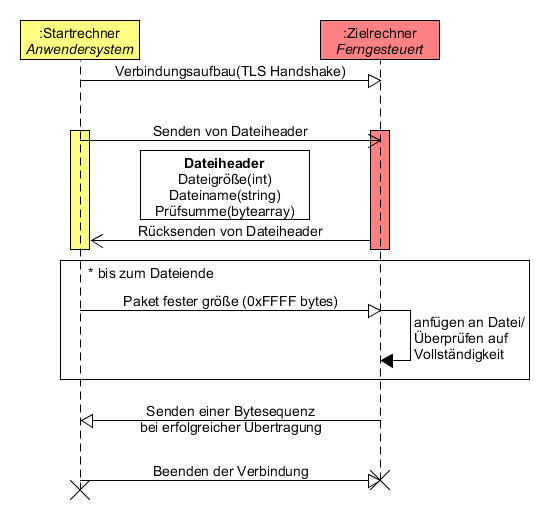
\includegraphics[scale=.4]{diagramFileProtocol}
\caption{Schematische Darstellung des Ablaufs bei der Dateiübertragung}
\label{file_diagram}
\end{wrapfigure}

Dieses Informationspaket ist in Abbildung \ref{Datei_Header} schematisch dargestellt.
Es besteht aus der Art der Datei (z.B. Video, Audio, Text, ausführbare Dateien etc.), was in der weiteren Einordnung im Zielcomputer nützlich ist, dem ursprünglichen Dateinamen und einer Prüfsumme, mit der die fehlerfreie Ankunft verifiziert werden kann. Auch hier spielt der tatsächliche Zahlenwert, der hinter dem Typ steht nur intern eine Rolle, abgesehen von benutzerdefinierten Erweiterungen. Deshalb sind die Codierungstabllen im Anhang nachzulesen. [s. S. \pageref{enums}]\\\\
Das Headersegment ist daher so aufgebaut, dass zunächst die drei Ganzzahlwerte für Typ, Länge des Dateinamen in Byte und Länge der Prüfsumme in Byte in den Header geschrieben werden. 
Dann werden die Länge des Dateinamens und Prüfsumme angehängt und dieses gesamte Paket wird an den Zielcomputer übermittelt.\par
Ist die Verbindung verifiziert, wird mit der eigentlichen Übertragung der Datei begonnen, die in kleinen Abschnitten und ohne weitere Kennzeichnung in mehreren kleinen Paketen geschieht.
Das funktioniert, da unser Standard zum Einen auf TCP/IP aufbaut, welcher bereits die richtige Reihenfolge und Vollständigkeit der Pakete weitgehend sicherstellt und zum Anderen nur eine Verbindung pro Dateiübertragung aktiv ist.
Am Zielcomputer wird die Datei schließlich in einem temporären Standardverzeichnis abgespeichert und Paket für Paket zusammengesetzt.
Ist die Übertragung nach dem Senden einer bestimmten Bytesequenz vom Zielcomputer beendet, wird ein Signal aus der Managerklasse ausgesendet und die Verbindung getrennt.
Diese Schrittfolge ist schematisch in Abbildung \ref{file_diagram} dargestellt.
Nach dem erfolgreichen Übertragen wird noch mit der anfänglich verschickten Prüfsumme der Datei die Integrität der Datei geprüft, um Fehler insgesamt auszuschließen, und die weitere Verarbeitung an die anderen Programmteile abgegeben.\\\\
Alle Anforderungen an das Protokoll werden erfüllt; der gesicherte und verschlüsselte Transport von Daten ist durch die Verwendung einer TLS-Verbindung und dem Aufbau eigener Kanäle erfüllt, die fehlerfreie Übertragung von Daten wird am Zielort über Gesamtgröße und Prüfsummen verifiziert, der Kommunikationskanal ist symmetrisch aufgebaut, da die Bibliothek sowohl für den Start- als auch für den Zielcomputer die nötige Funktionalität bereitstellt; die Codierung von allen Informationen als Zahlen oder als Bitflags sowie die Nutzung eigener Kanäle für Dateien reduziert den Datenverkehr drastisch, und damit ist auch dieser Punkt erfüllt, außerdem ist die Verwendung von Zahlencodes systematisch erweiterbar auf derselben Speicherbreite, also wurden alle Ziele erreicht.

\subsection{Funktionsumfang der selbstgeschriebenen Klassenbibliothek}
Die Bibliothek stellt auf oberster Ebene eine Schnittstelle zum Übertragen von Dateien und Anweisungen zu einer bekannten Netzwerkadresse.
Das heißt konkret, es werden Methoden bereitgestellt, welche die einzelnen Informationen intern in die zuvor spezifizierte Form umwandeln und verschicken, sowie am Zielcomputer wieder entpacken und an die weiteren Programmteile übergeben.
Zusätzlich dazu ist natürlich eine entsprechende Fehlerbehandlung bei Verbindungsabbrüchen, fehlerhaften Übertragungen oder internen Kommunikationsproblemen durch falsche Eingaben und die Möglichkeit eine Fortschrittsmeldung bei der Dateiübertragung implementiert.
Insgesamt muss der Programmierer also nur mit zwei Klassen interagieren, um die volle Funktionalität der Bibliothek ausnutzen, weshalb sich das gesamte Konstrukt sehr gut für weitere Verwendungen in flexiblen Kontexten der modularen Programmierung eignet.

\subsection{Implementierung und Funktionsweise der Klassenbibliothek}
In der Bibliothek sind neben den beiden oben beschriebenen Manager-Klassen (MngThManager für Dateien und MngFileManager für Dateien) mehrere andere Klassen definiert, welche von den jeweiligen Manager-Klassen aus aufgerufen und benutzt werden und dadurch eine darunterliegende Schicht bilden, die durch eine fest definierte Schnittstelle an den Rest des Programms angebunden werden.
Außerdem gibt es eine von allen Klassen benutzte Datei, in denen die Datenstrukturen und Datentypen, die in den Header der Pakete geschrieben werden, als C-Structs definiert sind und einige Funktionen, die häufig gebraucht werden (z.B. String-Vervielfältigung, oder eine Funktion zum errechnen der Dateiprüfsumme) deklariert.\par
Der Aufbau der Übertragung beider Datentypen, die verschickt werden, ähnelt sich bis zu einem gewissen Punkt - so haben beide eine eigene Klasse, in der intern die Objekte(Anweisungen und Dateizugriffsobjekte) gespeichert sind und verwaltet werden: (\textit{FileHansz} bzw. \textit{InstructionHansz}), sowie andere Klassen zum Verbindungsaufbau und dem Versand: Eine Klasse, die für das Annehmen von hereinkommenden Verbindungen zuständig ist und eine(bei Dateien zwei) Socket-Klassen, die sich um das Senden bzw. Empfangen von Daten kümmern, was in Abb. \ref{inst_d} bzw. \ref{file_d} vereinfacht schematisch dargestellt ist.\\\\

\begin{wrapfigure}{r}{.55\textwidth}
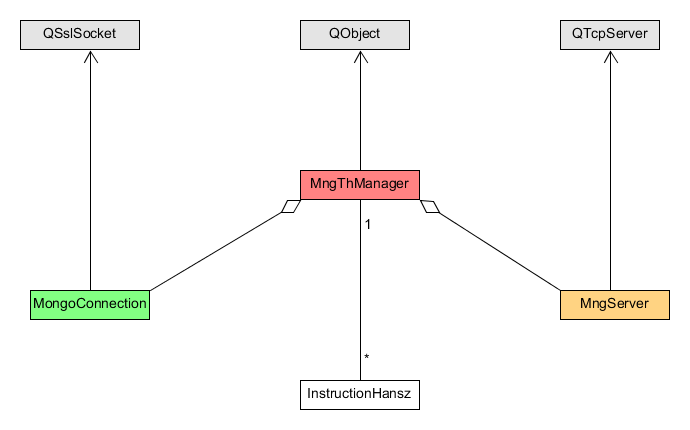
\includegraphics[scale=.4]{classDiagInstr}
\caption{Schematisch: Klassen zum Anweisungsversand}
\label{inst_d}
\end{wrapfigure}

Die beiden Speicherklassen werden dabei sowohl für den Empfang als auch das Senden eines Objektes genutzt - im ersten Fall werden sie mit den Teildaten(also Anweisungscode und zusätzlichen Argumenten oder Dateiname und Dateityp) initialisiert und erstellen daraus einen Pufferspeicher, der bereits den korrekten Header und das Datenpaket enthält, dessen Inhalt dann nur noch ausgelesen und verschickt werden muss - somit ist ein gleicher Aufbau der Verbindung in beide Richtungen sichergestellt.\par
Das tatsächliche Versenden, sowie der Verbindungsaufbau wird von einer "`Server"'-Klasse und den Socket-Klassen übernommen.
Dabei horcht die Serverklasse, sowohl für Dateien als auch für Anweisungen auf der Empfangenden Seite auf einem zuvor bestimmten Port auf eingehende Verbindungen.
Auf der sendenden Seite wird eine neue Klasse erstellt, welche ein TLS-Socket initialisiert und zu der gegebenen Adresse verbindet.
Ist die Verbindungsanfrage eingegangen, wird eine normale TLS-gesicherte Verbindung aufgebaut, sofern das möglich ist; danach weichen die Abläufe von Dateiversand und Anweisungsübertragung ab: Anweisungen werden jetzt, in der Reihenfolge in der sie eingehen, von der Managerklasse an das Socket getaktet weitergeleitet, wo sie dann inklusive Header und Datenpaket verschickt werden - bei Dateien ist der Ablauf etwas komplexer.\par

\begin{wrapfigure}{r}{.55\textwidth}
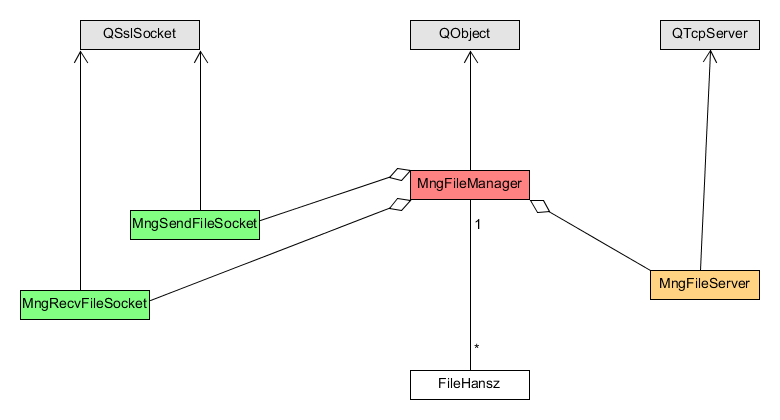
\includegraphics[scale=.35]{classDiagFile}
\caption{Schematisch: Klassen zum Dateiversand}
\label{file_d}
\end{wrapfigure}

Dabei muss zunächst erwähnt werden, dass für Dateien, im Gegensatz zu Anweisungen jedes Mal eine neue Verbindung aufgebaut wird.
In der Verbindung für eine Datei wird, sobald sie aufgebaut ist, zuerst der Header für die Dateiübertragung an den Zielcomputer gesendet, welcher genau dasselbe Paket dann zurückschickt um sicherzustellen, dass alle Steuerinformationen korrekt angekommen sind.
Jetzt wird die eigentliche Übertragung der Datei gestartet, welche mit dem Auslesen eines Datenblockes fester Größe beginnt.
Dieser wird in einen Pufferspeicher geschrieben, der, wenn er voll ist von der Socket-Klasse ausgelesen und übertragen wird; diese Anweisungsfolge wird so lange wiederholt, bis das Ende der Datei erreicht ist.
Der letzte Datenblock enthält oft weniger als die Maximalgröße, was aber in der Praxis kein Problem ist - das letzte Datenpaket auf der Seite des verschickenden Rechners ist nur etwas kleiner als der Rest.
Auf der empfangenden Seite werden die ankommenden Datenpakete über ihre Repräsentation als FileHansz-Objekt in eine nach der Datei-Prüfsumme benannten Datei im Dateisystem gespeichert - das verhindert die konkurrierende Benennung von ungleichen Dateien und vereinfacht das Überprüfen auf korrekte Übertragung; die ursprünglichen Namen werden zu Beginn der Übertragung per Signal an das Programm außerhalb der Bibliothek geschickt, welches diese dann weitergehend speichert - somit geht auch der Überblick nicht verloren.
Sind alle Pakete versandt worden und angekommen, wofür die TCP-basierte Verbindung sorgt, wird vom empfangenden Rechner eine Bytesequenz übertragen, welche die erfolgreiche Übertragung kennzeichnet.\par
Danach wird die Verbindung abgeschlossen und die beiden Sockets gelöscht.
Der gesamte Prozess ist in Abb. \ref{file_diagram} als Sequenzdiagramm dargestellt.\\
Die Verbindung für Anweisungen wird im Gegensatz erst am Programmende oder bei einem disconnect-Befehl getrennt; sie läuft auf Port 16962, die Dateiübertragung auf Port 16963.
Greift man über das Internet auf einen Computer in einem lokalen Netzwerk zu, so muss zuvor beim Standardgateway für beide Ports Port-Forwarding eingestellt werden.
%\end{document}